\documentclass[12pt,a4paper]{article}

% Pacotes
\usepackage[utf8]{inputenc}
\usepackage[T1]{fontenc}
\usepackage[brazilian]{babel}
\usepackage{amsmath, amssymb}
\usepackage{graphicx}
\usepackage{booktabs}
\usepackage{geometry}
\usepackage{float}
\usepackage{caption}
\usepackage{hyperref}
\usepackage{listings}
\usepackage{xcolor}

% Configuracao da pagina
\geometry{left=2.5cm, right=2.5cm, top=2.5cm, bottom=2.5cm}

% Configuracao de codigo Python
\lstdefinestyle{python}{
    language=Python,
    basicstyle=\ttfamily\small,
    keywordstyle=\color{blue},
    stringstyle=\color{red!70!black},
    commentstyle=\color{green!50!black},
    numbers=left,
    numberstyle=\tiny\color{gray},
    numbersep=5pt,
    frame=single,
    breaklines=true,
    showstringspaces=false
}

% ============================================================
\begin{document}

% Capa
\begin{titlepage}
\centering
\vspace*{2cm}

{\Large\textbf{Universidade Federal de Santa Catarina}}\\[0.3cm]
{\large Centro Tecnológico}\\[0.2cm]
{\large Departamento de Engenharia Elétrica e Eletrônica}\\[2cm]

{\LARGE\textbf{Trabalho I}}\\[0.5cm]
{\Large Despacho Econômico Simplificado}\\[2cm]

{\large\textbf{Disciplina:} EEL7833 -- Projeto em Sistemas de Energia II}\\[0.3cm]
{\large\textbf{Professor:} Erlon Cristian Finardi}\\[2cm]

{\large\textbf{Aluna:} Julia Pereira Madeira}\\[3cm]

{\large Florianópolis, agosto de 2026}

\end{titlepage}

% ============================================================
\section{Introdução}

Este trabalho apresenta a formulação e resolução de um problema de despacho econômico simplificado, no qual se busca determinar a alocação ótima de geração entre duas unidades termelétricas de forma a minimizar o custo total de operação, respeitando o atendimento à demanda e a manutenção de uma reserva de segurança operativa.

% ============================================================
\section{Dados do Problema}

O sistema é composto por duas unidades geradoras térmicas com as seguintes características:

\begin{table}[H]
\centering
\caption{Dados das unidades geradoras}
\begin{tabular}{@{}lccc@{}}
\toprule
Unidade & Custo variável (R\$/MWh) & Potência mínima (MW) & Potência máxima (MW) \\
\midrule
G1 & 150 & 0 & 80 \\
G2 & 220 & 0 & 70 \\
\bottomrule
\end{tabular}
\end{table}

\begin{itemize}
    \item Demanda mínima a ser atendida: 100 MW
    \item Reserva mínima de segurança: 10 MW
    \item Capacidade total instalada: $80 + 70 = 150$ MW
\end{itemize}

% ============================================================
\section{Formulação do Problema}

\subsection{Variáveis de Decisão}

\begin{itemize}
    \item $g_1$: potência gerada pela unidade G1 (MW)
    \item $g_2$: potência gerada pela unidade G2 (MW)
\end{itemize}

\subsection{Problema de Programação Linear}

\begin{align}
\min \quad & Z = 150\,g_1 + 220\,g_2 \label{eq:obj}\\[6pt]
\text{sujeito a:} \quad & g_1 + g_2 \geq 100 \quad \text{(atendimento à demanda)} \label{eq:demanda}\\
& g_1 + g_2 \leq 140 \quad \text{(reserva de segurança)} \label{eq:reserva}\\
& 0 \leq g_1 \leq 80 \quad \text{(limites de G1)} \label{eq:g1}\\
& 0 \leq g_2 \leq 70 \quad \text{(limites de G2)} \label{eq:g2}
\end{align}

\noindent A restrição \eqref{eq:reserva} decorre da exigência de reserva mínima de 10~MW: como a capacidade total instalada é 150~MW, a geração total não pode exceder $150 - 10 = 140$~MW.

% ============================================================
\section{Região Viável}

A região viável é o conjunto de pontos $(g_1, g_2)$ que satisfazem simultaneamente todas as restrições \eqref{eq:demanda}--\eqref{eq:g2}. Trata-se de um polígono convexo no primeiro quadrante, delimitado pelas retas:

\begin{itemize}
    \item $g_1 + g_2 = 100$ (fronteira inferior -- demanda)
    \item $g_1 + g_2 = 140$ (fronteira superior -- reserva)
    \item $g_1 = 80$ (limite de G1)
    \item $g_2 = 70$ (limite de G2)
\end{itemize}

A Figura~\ref{fig:regiao} apresenta a representação gráfica da região viável, os vértices e as curvas de isocusto.

\begin{figure}[H]
\centering
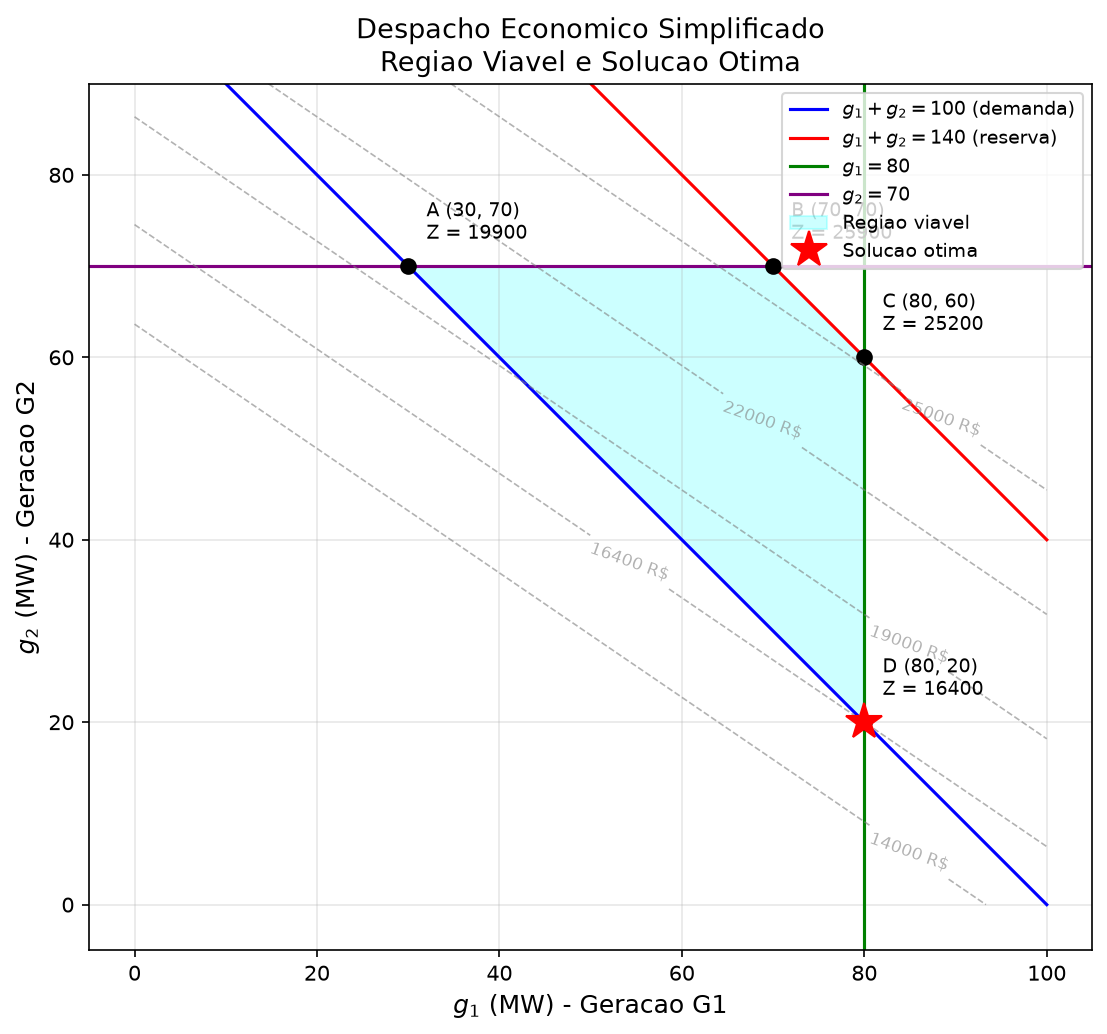
\includegraphics[width=0.85\textwidth]{regiao_viavel.png}
\caption{Região viável, vértices e solução ótima do problema de despacho econômico.}
\label{fig:regiao}
\end{figure}

% ============================================================
\section{Vértices da Região Viável}

Os vértices do polígono viável são determinados pelas interseções das restrições ativas:

\begin{table}[H]
\centering
\caption{Vértices da região viável e respectivos custos}
\begin{tabular}{@{}ccccc@{}}
\toprule
Vértice & $g_1$ (MW) & $g_2$ (MW) & Restrições ativas & $Z$ (R\$/h) \\
\midrule
A & 30 & 70 & $g_2 = 70$, $g_1 + g_2 = 100$ & 19.900 \\
B & 70 & 70 & $g_2 = 70$, $g_1 + g_2 = 140$ & 25.900 \\
C & 80 & 60 & $g_1 = 80$, $g_1 + g_2 = 140$ & 25.200 \\
D & 80 & 20 & $g_1 = 80$, $g_1 + g_2 = 100$ & \textbf{16.400} \\
\bottomrule
\end{tabular}
\end{table}

% ============================================================
\section{Solução Ótima}

A solução ótima ocorre no vértice D, onde a função objetivo atinge seu valor mínimo:

\begin{equation}
\boxed{g_1^* = 80 \text{ MW}, \quad g_2^* = 20 \text{ MW}, \quad Z^* = 16.400 \text{ R\$/h}}
\end{equation}

\begin{table}[H]
\centering
\caption{Resumo da solução ótima}
\begin{tabular}{@{}lc@{}}
\toprule
Grandeza & Valor \\
\midrule
Geração G1 & 80 MW \\
Geração G2 & 20 MW \\
Geração total & 100 MW \\
Reserva disponível & 50 MW \\
Custo total & 16.400 R\$/h \\
\bottomrule
\end{tabular}
\end{table}

% ============================================================
\section{Interpretação Física}

A solução ótima reflete o princípio fundamental do \textbf{despacho por ordem de mérito econômico}:

\begin{enumerate}
    \item A unidade G1, com menor custo variável (150~R\$/MWh), é despachada em sua \textbf{capacidade máxima} (80~MW).
    
    \item A unidade G2, mais cara (220~R\$/MWh), gera apenas o \textbf{complemento necessário} para atender à demanda mínima de 100~MW, resultando em $g_2 = 20$~MW.
    
    \item A geração total coincide exatamente com a demanda (100~MW), pois qualquer geração adicional apenas aumentaria o custo sem benefício operativo.
    
    \item A reserva disponível é de 50~MW, muito superior ao mínimo exigido de 10~MW. Isso ocorre naturalmente porque o atendimento da demanda no ponto ótimo já garante folga na restrição de reserva.
    
    \item As restrições ativas na solução ótima são: o limite máximo de G1 ($g_1 = 80$) e o atendimento à demanda ($g_1 + g_2 = 100$).
\end{enumerate}

\noindent Este resultado ilustra que, em problemas de despacho econômico, as unidades com menor custo variável devem ser priorizadas até sua capacidade máxima antes de acionar unidades mais caras.

% ============================================================
\section{Implementação Computacional}

O problema foi resolvido computacionalmente utilizando Python com a biblioteca \texttt{scipy.optimize.linprog}. O código também gera a representação gráfica da região viável. Os resultados computacionais confirmam a solução analítica obtida graficamente.

\begin{lstlisting}[style=python, caption={Trecho principal da implementação}]
from scipy.optimize import linprog

# Funcao objetivo: min 150*g1 + 220*g2
c = [150, 220]

# Restricoes (formato A_ub @ x <= b_ub)
A_ub = [[-1, -1],   # -g1 - g2 <= -100 (demanda)
         [1,  1]]   #  g1 + g2 <= 140  (reserva)
b_ub = [-100, 140]

# Limites das variaveis
bounds = [(0, 80), (0, 70)]

# Resolucao
result = linprog(c, A_ub=A_ub, b_ub=b_ub, bounds=bounds)
# Resultado: g1=80, g2=20, Z=16400
\end{lstlisting}

% ============================================================
\section{Conclusão}

O problema de despacho econômico simplificado foi formulado como um problema de Programação Linear com duas variáveis de decisão, resolvido tanto graficamente quanto computacionalmente. A solução ótima demonstra o princípio do despacho por mérito econômico: a unidade de menor custo opera na capacidade máxima, enquanto a unidade mais cara gera apenas o necessário para complementar a demanda. O custo mínimo de operação é de 16.400~R\$/h, com reserva de segurança de 50~MW — significativamente acima do mínimo exigido.

\end{document}
